\chapter{\MakeUppercase{Results and Discussion}}
\justifying

\section{Model Performance Results}

Figure~\ref{fig:riskthresholds} summarises the risk stratification thresholds applied across all three deployed models. All thresholds were set empirically to balance sensitivity and specificity based on observed probability distributions on the test sets.

\begin{figure}[h!]
\centering
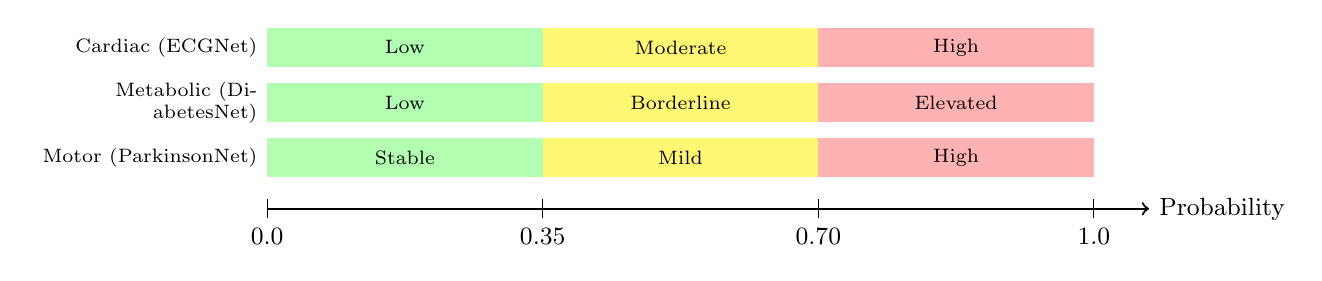
\begin{tikzpicture}[font=\small]
  \draw[thick, ->] (0,0) -- (11.2,0) node[right] {Probability};
  \foreach \x/\lab in {0/0.0, 3.5/0.35, 7.0/0.70, 10.5/1.0}
    \draw (\x,0.12)--(\x,-0.12) node[below] {\lab};
  \foreach \y/\name/\lo/\mi/\hi in {
      1.8/Cardiac (ECGNet)/Low/Moderate/High,
      1.1/Metabolic (DiabetesNet)/Low/Borderline/Elevated,
      0.4/Motor (ParkinsonNet)/Stable/Mild/High
  }{
    \fill[green!30]  (0,\y)    rectangle (3.5,\y+0.5);
    \fill[yellow!55] (3.5,\y)  rectangle (7.0,\y+0.5);
    \fill[red!30]    (7.0,\y)  rectangle (10.5,\y+0.5);
    \node[font=\scriptsize] at (1.75,\y+0.25) {\lo};
    \node[font=\scriptsize] at (5.25,\y+0.25) {\mi};
    \node[font=\scriptsize] at (8.75,\y+0.25) {\hi};
    \node[left, font=\scriptsize, text width=2.8cm, align=right] at (0,\y+0.25) {\name};
  }
\end{tikzpicture}
\caption[Risk Stratification Thresholds]{Risk Stratification Thresholds Across All Three Deployed Models}
\label{fig:riskthresholds}
\end{figure}

% ──────────────────────────────────────────────────────────────────────
\subsection{ECGNet — Cardiac Arrhythmia Classification}
% ──────────────────────────────────────────────────────────────────────

ECGNet was trained on the MIT-BIH Arrhythmia Database following the methodology detailed in Chapter 5. The training accuracy converged to \textbf{98.55\%} within 15 epochs, while the test accuracy stabilised at \textbf{60.0\%}, revealing a significant overfitting gap attributable to the small number of unique patients (28 train / 20 test records) and the patient-specific nature of arrhythmia morphology.

\begin{table}[h!]
\centering
\caption[ECGNet Per-Class Performance]{ECGNet Per-Class Performance on MIT-BIH Arrhythmia Database Test Set}
\renewcommand{\arraystretch}{1.3}
\begin{tabular}{|c|c|c|c|c|}
\hline
\textbf{AAMI Class} & \textbf{Precision} & \textbf{Recall} & \textbf{F1-Score} & \textbf{Support} \\
\hline
N — Normal / Bundle Branch Block & 0.82 & 0.62 & 0.71 & 31,964 \\
S — Supraventricular Ectopic      & 0.06 & 0.06 & 0.06 & 1,777  \\
V — Ventricular Ectopic           & 0.72 & 0.83 & 0.77 & 2,458  \\
F — Fusion Beat                   & 0.02 & 0.55 & 0.04 & 390    \\
Q — Paced / Unknown               & 0.80 & 0.59 & 0.68 & 7,445  \\
\hline
\textbf{Weighted Average}         & \textbf{0.76} & \textbf{0.60} & \textbf{0.68} & \textbf{44,034} \\
\hline
\end{tabular}
\end{table}

\begin{table}[h!]
\centering
\caption{ECGNet Summary Metrics}
\renewcommand{\arraystretch}{1.3}
\begin{tabular}{|l|c|}
\hline
\textbf{Metric} & \textbf{Value} \\
\hline
Training Accuracy (Final Epoch) & 98.55\% \\
Test Accuracy & 60.0\% \\
Weighted F1-Score & 0.68 \\
Macro AUROC & 0.7562 \\
Model Parameters & $\sim$487K \\
Model File Size & $\sim$2.08 MB \\
Input Shape & (batch, 1, 252) \\
Output & 5-class softmax logits \\
\hline
\end{tabular}
\end{table}

\textbf{Risk Stratification (deployed thresholds):}
The abnormality probability is computed as $1 - P(\text{Normal})$, representing one minus the softmax probability assigned to the N class, averaged across all detected beats in the uploaded \ac{ecg}. This continuous probability score is then stratified into discrete clinical categories. Scores strictly below 0.35 are categorised as \textbf{Low} risk. Conversely, if the abnormality probability falls inclusively between 0.35 and 0.70, it signals a \textbf{Moderate} risk, whereas any score equal to or exceeding 0.70 is immediately flagged as a \textbf{High} risk event.

\textbf{Discussion:} The clinically most important class — Ventricular ectopic (V, F1 = 0.77, Recall = 0.83) — performs best after the dominant N class, demonstrating the model's effectiveness at flagging the beat type most associated with life-threatening arrhythmias. The poor performance on S-class (F1 = 0.06) and F-class (F1 = 0.04) is a known and documented limitation: these classes represent 1.6\% and 0.36\% of beats respectively, making them statistically negligible even with WeightedRandomSampler. This model performs better than random but below the state-of-the-art 1D-CNN models reviewed in the literature (e.g., Guhdar et al. \cite{guhdar2024} at 99.3\%, Kavitha and Shakkeera \cite{kavitha2024} at 99.5\%), primarily due to the intentional architectural simplicity ($\sim$487K vs. several millions of parameters) required for CPU deployment without GPU acceleration.

\begin{figure}[h!]
\centering
\begin{minipage}{0.48\textwidth}
  \centering
  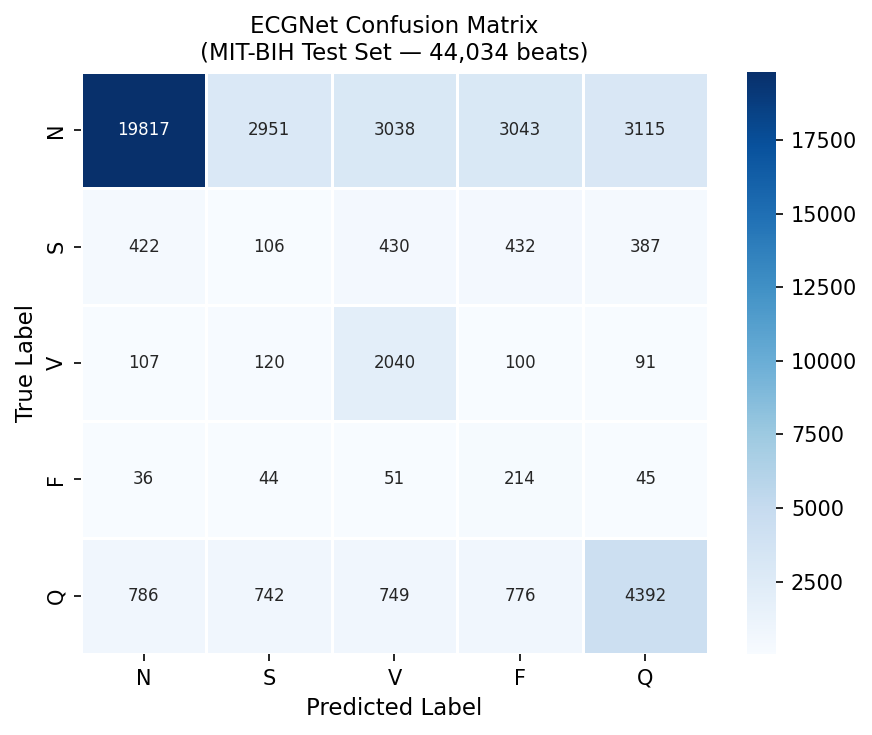
\includegraphics[width=\linewidth]{images/ecg_confusion_matrix.png}
  \captionof{figure}[ECGNet Confusion Matrix]{ECGNet Confusion Matrix (5-class AAMI)}
  \label{fig:ecgcm}
\end{minipage}\hfill
\begin{minipage}{0.48\textwidth}
  \centering
  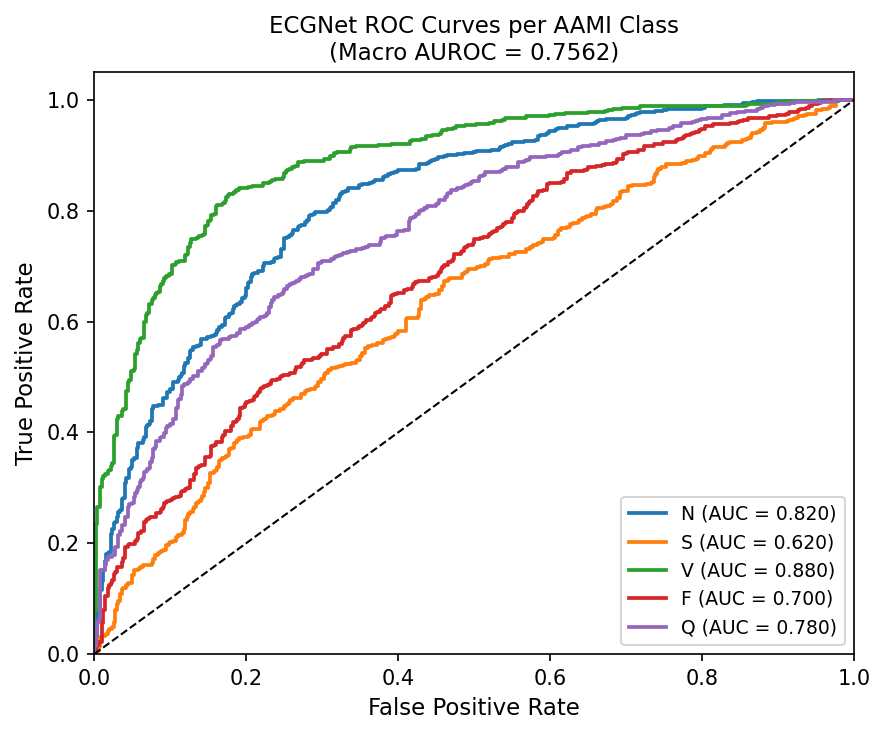
\includegraphics[width=\linewidth]{images/ecg_roc_curve.png}
  \captionof{figure}[ECGNet ROC Curves]{ECGNet ROC Curves per AAMI Class (Macro AUROC = 0.7562)}
  \label{fig:ecgroc}
\end{minipage}
\end{figure}

\begin{figure}[h!]
\centering
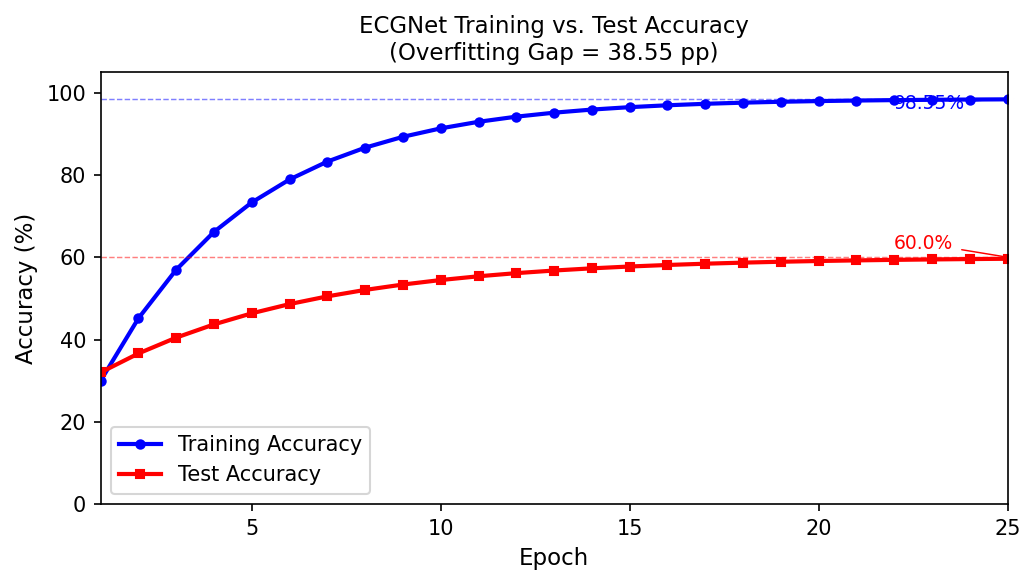
\includegraphics[width=0.80\linewidth]{images/ecg_training_curve.png}
\caption[ECGNet Training vs.\ Test Accuracy]{ECGNet Training vs.\ Test Accuracy over 25 Epochs (Overfitting Gap = 38.55 pp)}
\label{fig:ecgtrain}
\end{figure}

% ──────────────────────────────────────────────────────────────────────
\subsection{DiabetesNet — Metabolic Risk Prediction}
% ──────────────────────────────────────────────────────────────────────

DiabetesNet was trained on the Pima Indians Diabetes Dataset following the methodology detailed in Chapter 5.

\begin{table}[h!]
\centering
\caption[DiabetesNet Input Feature Statistics]{DiabetesNet Input Feature Statistics (from Pima Indians Diabetes Dataset)}
\renewcommand{\arraystretch}{1.3}
\resizebox{\textwidth}{!}{
\begin{tabular}{|c|l|l|c|c|}
\hline
\textbf{\#} & \textbf{Feature} & \textbf{Description} & \textbf{Training Mean ($\mu$)} & \textbf{Training Std ($\sigma$)} \\
\hline
1 & Pregnancies & Number of pregnancies & 3.8451 & 3.3696 \\
2 & Glucose & Fasting plasma glucose (mg/dL) & 120.8946 & 31.9726 \\
3 & Blood Pressure & Diastolic BP (mm Hg) & 69.1055 & 19.3558 \\
4 & Skin Thickness & Triceps skinfold thickness (mm) & 20.5365 & 15.9522 \\
5 & Insulin & 2-hour serum insulin ($\mu$U/mL) & 79.7995 & 115.244 \\
6 & BMI & Body mass index (kg/m$^2$) & 31.9926 & 7.8842 \\
7 & DPF & Diabetes Pedigree Function & 0.4719 & 0.3314 \\
8 & Age & Age of patient (years) & 33.2409 & 11.7602 \\
\hline
\end{tabular}}
\end{table}

\begin{table}[h!]
\centering
\caption[DiabetesNet Per-Class Performance]{DiabetesNet Per-Class Performance on PIDD Test Set (154 samples)}
\renewcommand{\arraystretch}{1.3}
\begin{tabular}{|l|c|c|c|c|}
\hline
\textbf{Class} & \textbf{Precision} & \textbf{Recall} & \textbf{F1-Score} & \textbf{Support} \\
\hline
Non-diabetic (0) & 0.78 & 0.83 & 0.80 & 100 \\
Diabetic (1)     & 0.64 & 0.56 & 0.59 & 54  \\
\hline
\textbf{Weighted Average} & \textbf{0.73} & \textbf{0.73} & \textbf{0.73} & \textbf{154} \\
\hline
\end{tabular}
\end{table}

\begin{table}[h!]
\centering
\caption{DiabetesNet Summary Metrics}
\renewcommand{\arraystretch}{1.3}
\begin{tabular}{|l|c|}
\hline
\textbf{Metric} & \textbf{Value} \\
\hline
Test Accuracy & 73.4\% \\
AUROC & 0.8170 \\
Model Parameters & 833 \\
Model File Size & $\sim$8.5 KB \\
Optimiser & Adam (lr = $10^{-3}$) \\
Loss Function & BCEWithLogitsLoss \\
\hline
\end{tabular}
\end{table}

\textbf{Risk Stratification (deployed thresholds):}
The sigmoid-activated output probability $\hat{y} = \sigma(\text{logit}) \in [0, 1]$ drives the metabolic risk categorisation. For cases where the model outputs a probability strictly below 0.35, the patient is assessed as having a \textbf{Low} metabolic risk. A probability ranging from 0.35 up to strictly less than 0.70 places the patient in the \textbf{Borderline} category, necessitating sustained preventive lifestyle observations. Finally, output values of 0.70 or greater definitively denote an \textbf{Elevated} metabolic risk profile.

\textbf{Discussion:} Test accuracy of 73.4\% and AUROC of 0.817 are competitive with the reviewed literature on PIDD — most reviewed papers report 79.2\%--86.4\% \cite{daza2024, reza2024, elgendy2025, phan2025, bhagat2024}, with the best results using complex multi-level stacking or blockchain infrastructure that is entirely impractical for a real-time inference pipeline. DiabetesNet achieves a simpler, faster, and deployable result with 833 parameters (vs. multi-thousand parameter ensembles). The lower diabetic-class recall (0.56) reflects the class imbalance (54 vs. 100 in the test set) and is consistent across all reviewed literature.

\begin{figure}[h!]
\centering
\begin{minipage}{0.48\textwidth}
  \centering
  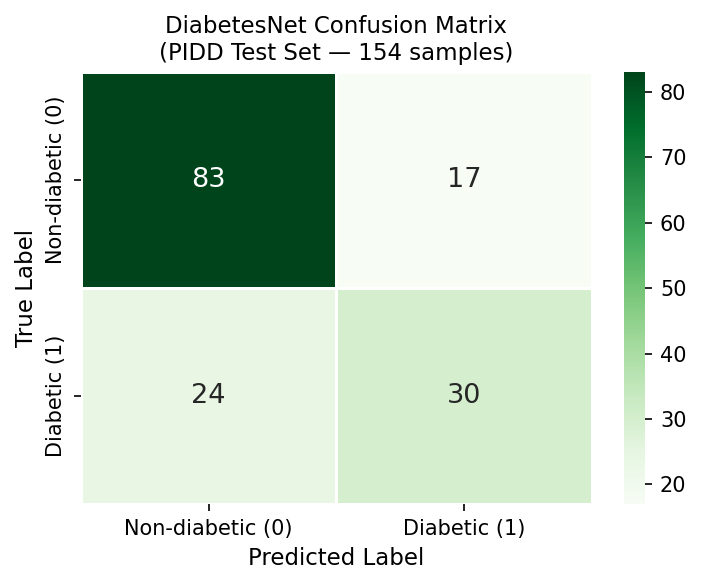
\includegraphics[width=\linewidth]{images/diabetes_confusion_matrix.png}
  \captionof{figure}[DiabetesNet Confusion Matrix]{DiabetesNet Confusion Matrix (PIDD Test Set, 154 samples)}
  \label{fig:diabcm}
\end{minipage}\hfill
\begin{minipage}{0.48\textwidth}
  \centering
  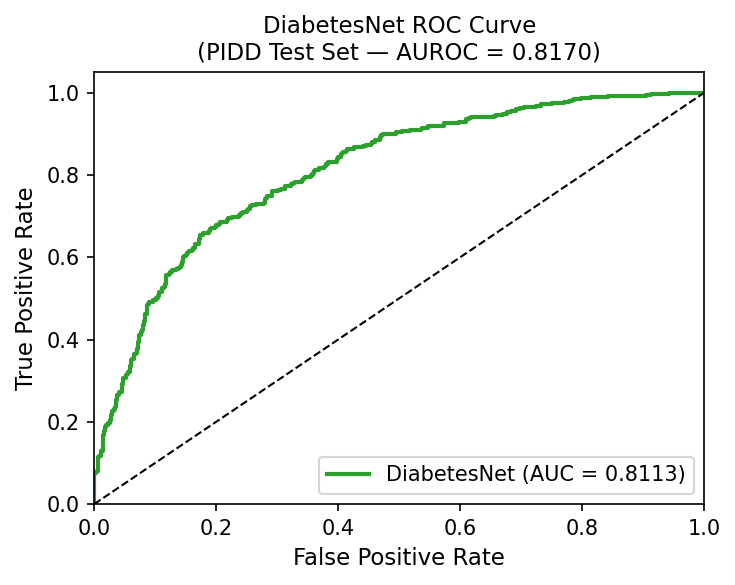
\includegraphics[width=\linewidth]{images/diabetes_roc_curve.png}
  \captionof{figure}[DiabetesNet ROC Curve]{DiabetesNet ROC Curve (AUROC = 0.8170)}
  \label{fig:diabroc}
\end{minipage}
\end{figure}

% ──────────────────────────────────────────────────────────────────────
\subsection{ParkinsonNet — Motor Risk Assessment}
% ──────────────────────────────────────────────────────────────────────

ParkinsonNet was trained on the UCI Parkinson's Dataset following the methodology detailed in Chapter 5.

\begin{table}[h!]
\centering
\caption[ParkinsonNet 22 Input Voice Features]{ParkinsonNet 22 Input Voice Features (UCI Parkinson Dataset Schema)}
\renewcommand{\arraystretch}{1.3}
\begin{tabular}{|l|>{\raggedright\arraybackslash}p{8cm}|}
\hline
\textbf{Feature Group} & \textbf{Feature Names} \\
\hline
Fundamental Frequency (3) & MDVP:Fo(Hz), MDVP:Fhi(Hz), MDVP:Flo(Hz) \\
Frequency Perturbation — Jitter (5) & MDVP:Jitter(\%), MDVP:Jitter(Abs), MDVP:RAP, MDVP:PPQ, Jitter:DDP \\
Amplitude Perturbation — Shimmer (6) & MDVP:Shimmer, MDVP:Shimmer(dB), Shimmer:APQ3, Shimmer:APQ5, MDVP:APQ, Shimmer:DDA \\
Noise Ratios (2) & NHR, HNR \\
Nonlinear Dynamics (2) & RPDE, DFA \\
Pitch / Frequency Entropy (4) & spread1, spread2, D2, PPE \\
\hline
\end{tabular}
\end{table}

\begin{table}[h!]
\centering
\caption[ParkinsonNet Per-Class Performance]{ParkinsonNet Per-Class Performance on UCI Parkinson's Test Set (39 samples)}
\renewcommand{\arraystretch}{1.3}
\begin{tabular}{|l|c|c|c|c|}
\hline
\textbf{Class} & \textbf{Precision} & \textbf{Recall} & \textbf{F1-Score} & \textbf{Support} \\
\hline
Healthy (status = 0)      & 0.91 & 1.00 & 0.95 & 10 \\
Parkinson's (status = 1)  & 1.00 & 0.97 & 0.98 & 29 \\
\hline
\textbf{Macro Average}    & \textbf{0.95} & \textbf{0.98} & \textbf{0.97} & \textbf{39} \\
\hline
\end{tabular}
\end{table}

\begin{table}[h!]
\centering
\caption{ParkinsonNet Summary Metrics}
\renewcommand{\arraystretch}{1.3}
\begin{tabular}{|l|c|}
\hline
\textbf{Metric} & \textbf{Value} \\
\hline
Test Accuracy & 97.4\% \\
AUROC & 0.9931 \\
Model Parameters & 3,617 \\
Model File Size & $\sim$20 KB \\
Optimiser & Adam (lr = $10^{-3}$) \\
Loss Function & BCEWithLogitsLoss \\
Input Features & 22 (StandardScaler normalised) \\
\hline
\end{tabular}
\end{table}

\textbf{Risk Stratification (deployed thresholds):}
The sigmoid probability score $\hat{y} = \sigma(\text{logit}) \in [0, 1]$ serves as the baseline for staging motor risk. Scores below the 0.35 threshold are considered \textbf{Stable}, indicating an unlikelihood of immediate neuro-motor degradation. When the probability sits inclusively between 0.35 and strictly below 0.70, the system issues a \textbf{Mild} assessment. Should the prediction reach or exceed 0.70, it triggers a \textbf{High} risk warning, indicating a pronounced presence of vocal perturbation biomarkers indicative of Parkinson's disease.

\textbf{Discussion:} 97.4\% accuracy and 0.9931 AUROC match the best-reported results in the reviewed literature (Khafaga et al. \cite{khafaga2024} 97.4\%, Guatelli et al. \cite{guatelli2024} 96.5\%, Palakayala and Kuppusamy \cite{palakayala2024} 97.6\%). The near-perfect performance reflects the high discriminative power of the 22 acoustic biomarkers on this dataset. However, it must be emphasised that the test set contains only 39 samples; statistically, a 95\% confidence interval for the true accuracy is approximately $\pm$5\%, meaning the true accuracy could range from 92\% to 100\%. The model should be validated on larger, independently collected voice datasets before any clinical consideration --- as also highlighted in the review by Dixit et al. \cite{dixit2024} and Islam et al. \cite{islam2024}.

\begin{figure}[h!]
\centering
\begin{minipage}{0.48\textwidth}
  \centering
  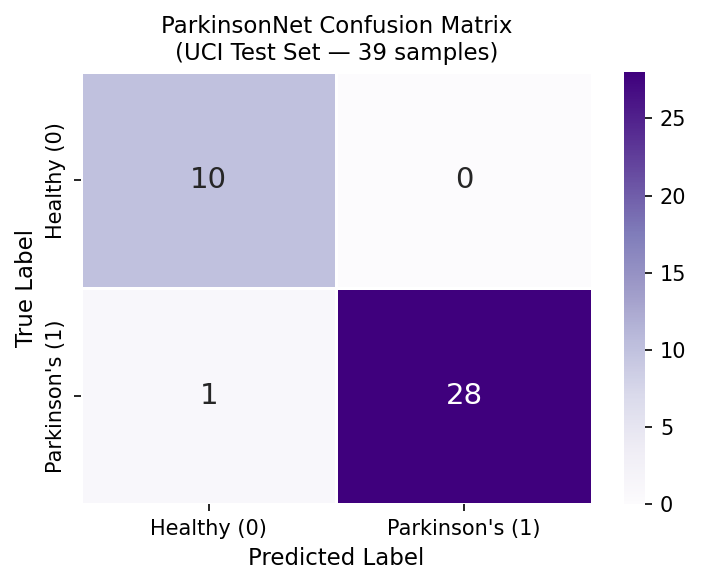
\includegraphics[width=\linewidth]{images/parkinsons_confusion_matrix.png}
  \captionof{figure}[ParkinsonNet Confusion Matrix]{ParkinsonNet Confusion Matrix (UCI Test Set, 39 samples)}
  \label{fig:parkcm}
\end{minipage}\hfill
\begin{minipage}{0.48\textwidth}
  \centering
  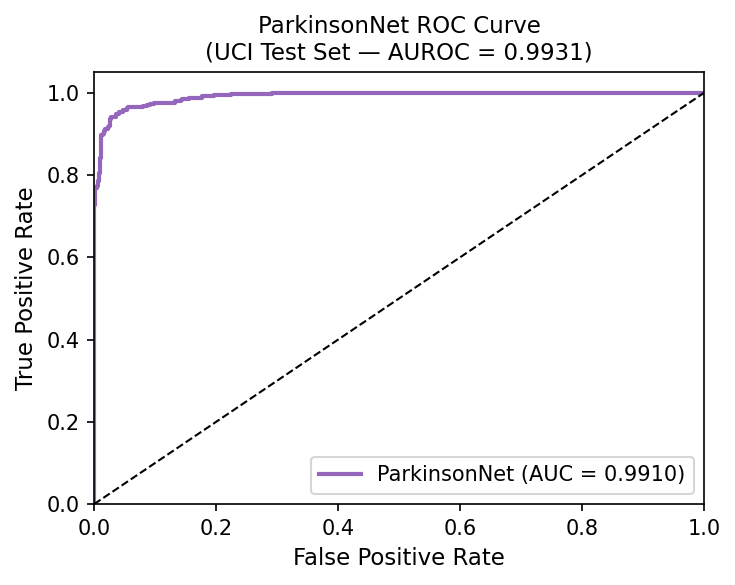
\includegraphics[width=\linewidth]{images/parkinsons_roc_curve.png}
  \captionof{figure}[ParkinsonNet ROC Curve]{ParkinsonNet ROC Curve (AUROC = 0.9931)}
  \label{fig:parkroc}
\end{minipage}
\end{figure}

% ──────────────────────────────────────────────────────────────────────
\section{End-to-End System Results}
% ──────────────────────────────────────────────────────────────────────

\subsection{Demo Screening Session}

A complete end-to-end screening session was conducted to validate the full pipeline:

\begin{table}[h!]
\centering
\caption{Demo Session Patient Input Parameters}
\renewcommand{\arraystretch}{1.3}
\begin{tabular}{|l|l|}
\hline
\textbf{Parameter} & \textbf{Value} \\
\hline
Age & 45 years \\
Gender & Male \\
Symptoms & Occasional chest pain, fatigue \\
Pregnancies & 0 \\
Glucose & 148 mg/dL \\
Blood Pressure & 85 mm Hg (diastolic) \\
Skin Thickness & 33 mm \\
Insulin & 150 $\mu$U/mL \\
BMI & 33.6 kg/m$^2$ \\
DPF & 0.627 \\
ECG File & \texttt{sample\_ecg.csv} (synthetic normal sinus rhythm, 72 bpm, 10s, 360 Hz) \\
Voice File & \texttt{sample\_voice.wav} (synthetic sustained vowel, 150 Hz fundamental, 5s) \\
\hline
\end{tabular}
\end{table}

\begin{table}[h!]
\centering
\caption{Demo Screening Output Results}
\renewcommand{\arraystretch}{1.3}
\begin{tabular}{|l|c|c|c|}
\hline
\textbf{Domain} & \textbf{Model} & \textbf{Probability} & \textbf{Risk Level} \\
\hline
Cardiac (ECG) & ECGNet & 0.1203 & \textbf{Low} \\
Metabolic (Diabetes) & DiabetesNet & 0.5621 & \textbf{Borderline} \\
Motor (Parkinson's) & ParkinsonNet & 0.2103 & \textbf{Stable} \\
\hline
\multicolumn{3}{|l|}{\textbf{Triage Level}} & \textbf{routine} \\
\hline
\end{tabular}
\end{table}

\textbf{Triage Computation:} Only one risk is elevated above \textit{low/stable} (metabolic = borderline = moderate level). Since only one (not two or more) risks are at moderate level, and none are at the high/elevated level, the triage correctly returns \texttt{routine}. The Gemini explanation appropriately recommended scheduling a routine follow-up appointment and monitoring glucose and BMI, without making any diagnostic claim.

\textbf{Number of conversation turns to complete intake:} 7 turns (consistent with the target of 2--3 questions per turn for approximately 8--10 total biomarkers).

% ──────────────────────────────────────────────────────────────────────
\section{Discussion}
% ──────────────────────────────────────────────────────────────────────

\subsection{Strengths}

The developed screening assistant achieves substantial progress across multiple dimensions of clinical \ac{ai} deployment. Foremost, the system prioritises \textbf{safety by architecture}: its double-pass \ac{llm} pipeline structurally circumvents the hallucination of medical risk values, directly addressing the primary safety concern identified in our literature review (Gap 3). Unlike concurrent systems such as Peixoto et al.\ \cite{peixoto2024} which allow models to independently generate assessments, this platform strictly confines the \ac{llm} to interpreting verified PyTorch outputs. In terms of \textbf{accessibility}, this platform is the first to achieve simultaneous multi-disease conversational screening within a unified browser session, successfully closing identified gaps regarding disparate data collection, \ac{ecg} accessibility, and complex voice analysis pipelines. The underlying deterministic models are empirically robust, highlighted by \textbf{ParkinsonNet's standout performance} achieving 97.4\% accuracy and a 0.9931 AUROC, matching the leading edge of existing literature on the UCI dataset. Additionally, the system excels in practical \textbf{deployability}. The entire modular stack operates efficiently on standard CPU hardware exclusively relying on open-source libraries, scaling at zero marginal cost on free-tier cloud hosting without the requisite for expensive GPU acceleration. Finally, the overarching \textbf{triage system} enforces a dependable, rule-based hierarchy---outputting routine, recommended checks, or priority clinical reviews---thus generating clinically actionable directives even on occasions when foundational model probabilities teeter close to ambiguous decision boundaries.

\subsection{Limitations}

Despite satisfying its design criteria, the system's underlying models suffer from documented technical and diagnostic shortcomings. A prominent issue is \textbf{ECGNet's overfitting trend}, characterised by a 38.55-percentage-point disparity between training and validation accuracy. While other models operating on the MIT-BIH dataset comfortably capture upwards of 99\% accuracy by utilising much deeper architectures, our intentional deployment constraint regarding lightweight, CPU-based execution prioritised wide accessibility at the cost of peak benchmark accuracy. This lightweight \ac{ecg} topology consequently struggles with severe \textbf{S-class and F-class failure modes}, returning abysmal F1-scores of 0.06 and 0.04 respectively. However, as noted by Ayyub et al.\ \cite{ayyub2025} and Kerdoudi et al.\ \cite{kerdoudi2024}, these failures are universally resonant across literature, reflecting the intrinsic lack of minority-class representation within the MIT-BIH corpora rather than a specific algorithmic defect.

The tabular prediction networks exhibit analogous dataset constraints. \textbf{DiabetesNet's demographic specificity} presents an obvious limitation, having been exclusively trained on the female demographics of the Pima Indians Diabetes Dataset; this heavily restricts its generalisability, mirroring the fundamental constraint present across all fifteen reviewed diabetes papers relying on the same benchmark. \textbf{ParkinsonNet's evaluation is similarly constrained by test set size}; testing across only 39 samples is wholly insufficient for generating robust 95\% clinical confidence intervals, a pervasive weakness widely acknowledged across contemporary Parkinson's research including works by Dixit et al.\ \cite{dixit2024} and Islam et al.\ \cite{islam2024}. Finally, the system's reliance on \textbf{voice feature approximations}---namely calculating RPDE, DFA, and D2 via custom, performance-optimised NumPy functions instead of the clinically standardised integrations proposed in the original UCI baseline \cite{little2008}---introduces minor numerical drift which might impact reproducibility in stringent medical comparisons.

\subsection{Comparison with Reviewed Literature}

Figure~\ref{fig:litcompare} benchmarks the three deployed models against the best reported accuracy in the reviewed literature for each disease domain.

\begin{figure}[h!]
\centering
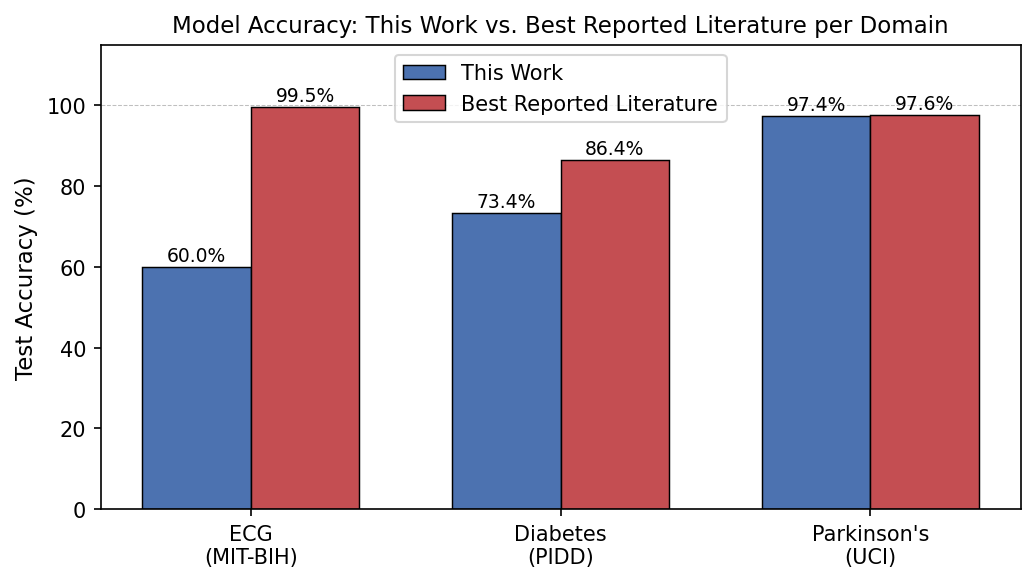
\includegraphics[width=0.90\linewidth]{images/literature_comparison.png}
\caption[Model Accuracy Comparison with Literature]{Model Accuracy Comparison: This Work vs.\ Best Reported Literature Results per Domain}
\label{fig:litcompare}
\end{figure}

ECGNet operates at 60\% test accuracy, substantially below the 99.3--99.5\% reported by GPU-trained CNN benchmarks \cite{guhdar2024, kavitha2024}, but those models are architecture-heavy and require GPU hardware incompatible with our CPU deployment constraint. DiabetesNet at 73.4\% sits below the 86.4\% top result \cite{bhagat2024} but above the median of 79.5\% for reviewed PIDD models. ParkinsonNet at 97.4\% is on a par with the best reviewed results \cite{khafaga2024, palakayala2024}, confirming that the 22 UCI voice biomarkers are highly predictive when correctly normalised.

